\documentclass[11pt]{article}
%\usepackage{alltt}
\usepackage[utf8]{inputenc}
\usepackage[dvips]{graphicx}
%\usepackage{a4wide}
\usepackage{epsfig}
\usepackage{fancybox}
\usepackage{verbatim}
\usepackage{array}
\usepackage{latexsym}
\usepackage{alltt}
%\usepackage{dsfont}

%\usepackage{fullpage}
\usepackage{hyperref}
\usepackage{textcomp}
\usepackage{listings}
\usepackage{color}
\usepackage{amsmath}
\usepackage{amsfonts}
\usepackage{tikz}
\usepackage{float}
\usepackage[hmargin=3cm,vmargin=5.0cm]{geometry}
%\topmargin=0cm
\topmargin=-1.8cm
\addtolength{\textheight}{6.5cm}
\addtolength{\textwidth}{2.0cm}
%\setlength{\leftmargin}{-5cm}
\setlength{\oddsidemargin}{0.0cm}
\setlength{\evensidemargin}{0.0cm}

\newcommand{\HRule}{\rule{\linewidth}{1mm}}
\newcommand{\kutu}[2]{\framebox[#1mm]{\rule[-2mm]{0mm}{#2mm}}}
\newcommand{\gap}{ \\[1mm] }

\newcommand{\Q}{\raisebox{1.7pt}{$\scriptstyle\bigcirc$}}

\lstset{
    %backgroundcolor=\color{lbcolor},
    tabsize=2,
    language=TeX,
    basicstyle=\footnotesize,
    numberstyle=\footnotesize,
    aboveskip={0.0\baselineskip},
    belowskip={0.0\baselineskip},
    columns=fixed,
    showstringspaces=false,
    breaklines=true,
    prebreak=\raisebox{0ex}[0ex][0ex]{\ensuremath{\hookleftarrow}},
    %frame=single,
    showtabs=false,
    showspaces=false,
    showstringspaces=false,
    identifierstyle=\ttfamily,
    keywordstyle=\color[rgb]{0,0,1},
    commentstyle=\color[rgb]{0.133,0.545,0.133},
    stringstyle=\color[rgb]{0.627,0.126,0.941},
}


\begin{document}



\section*{Question 1 \hfill \normalfont{(15 pts)}}
Let $S$ be a set of binary strings and $R$ be a relation on $S \times S$, defined as
\begin{align*}
\centering
S &= \{w \;:\; w \textrm{is a binary string} , \, |w| \leq 3 \, , \, |n_0(w) - n_1(w) |\leq 1\,,\,\textrm{and } w \textrm{does not begin and does not end with } 00\}\\
R &= \{(w_1, w_2)\;:\; w_1 \in S\,,\,w_2 \in S\,\,\textrm{and } w_1 \textrm{is a substring of } w_2\}
\end{align*}
where $|w|$ denotes the length of the string $w$, $n_0(w)$ and $n_1(w)$ are functions that map input strings $w$ to the number of 0\textquotesingle s and 1\textquotesingle s in $w$, respectively. Also, use the convention that $w_1$ is a substring of $w_2$ if and only if $w_1$ is contained entirely within $w_2$ for any given strings $w_1$ and $w_2$. 
\begin{itemize}
	\item[\textbf{a.}] Draw $R$ as a directed graph. \hfill \normalfont{(2 pts)}
	\item[\textbf{b.}] Prove that $(S,R)$ is a poset. \hfill \normalfont{(4 pts)}
	\item[\textbf{c.}] Is $(S,R)$ a total order? Prove your answer. \hfill \normalfont{(3 pts)}
	\item[\textbf{d.}] Draw a Hasse diagram for $(S,R)$. State the maximal and minimal elements. \hfill \normalfont{(4 pts)}
	\item[\textbf{e.}] Identify whether $(S,R)$ constitutes a lattice or not. \hfill \normalfont{(2 pts)}
\end{itemize}

\section*{Question 2 \hfill \normalfont{(24 pts)}}
Given the directed graph $G$ in Figure~\ref{g2}, answer the questions.
\begin{figure}[H]
	\centering
	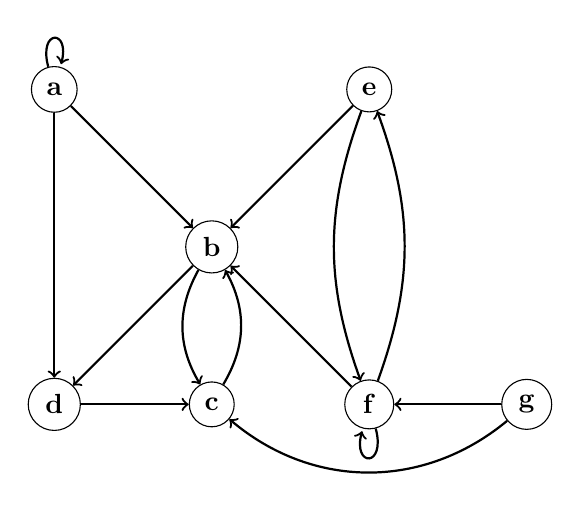
\begin{tikzpicture}
	
	\node[shape=circle,draw=black] (a) at (0, 4)     {\textbf{a}};
	\node[shape=circle,draw=black] (b) at (2, 2)     {\textbf{b}};
	\node[shape=circle,draw=black] (c) at (2, 0)     {\textbf{c}};
	\node[shape=circle,draw=black] (d) at (0, 0)     {\textbf{d}};
	\node[shape=circle,draw=black] (e) at (4, 4)     {\textbf{e}};
	\node[shape=circle,draw=black] (f) at (4, 0)     {\textbf{f}};
	\node[shape=circle,draw=black] (g) at (6, 0)     {\textbf{g}};

	\path[->, thick] (a) edge [loop above] (a);
	\path[->, thick] (a) edge (d);
	\path[->, thick] (a) edge (b);
	\path[->, thick] (b) edge (d);
	\path[->, thick] (b) edge [bend right=30] (c);
	\path[->, thick] (c) edge [bend right=30] (b);
	\path[->, thick] (d) edge (c);
	\path[->, thick] (e) edge (b);
	\path[->, thick] (e) edge [bend right=20] (f);
	\path[->, thick] (f) edge [bend right=20] (e);
	\path[->, thick] (f) edge [loop below] (f);
	\path[->, thick] (f) edge (b);
	\path[->, thick] (g) edge (f);
	\path[->, thick] (g) edge [bend left=40] (c);
	
	\end{tikzpicture} 
	\caption{Graph G in Q2.}	
	\label{g2}
\end{figure}

\begin{itemize}
	\item[\textbf{a.}] Provide an adjacency list representation of $G$. \hfill \normalfont{(3 pts)} 
	\item[\textbf{b.}] Provide an adjaceny matrix representation of $G$. \hfill \normalfont{(3 pts)}
	\item[\textbf{c.}] Compute indegrees and outdegrees of every vertex in $V$. \hfill \normalfont{(3 pts)}
	\item[\textbf{d.}] List $6$ different simple paths of length $4$ in $G$. \hfill \normalfont{(3 pts)}
	\item[\textbf{e.}] List all simple circuits of length $3$ in $G$. \hfill \normalfont{(3 pts)}
	\item[\textbf{f.}] Prove that $G$ is weakly-connected. \hfill \normalfont{(3 pts)}
	\item[\textbf{g.}] Identify strongly-connected components of $G$. \hfill \normalfont{(3 pts)}
	\item[\textbf{h.}] How many different paths of length $3$ exist between every distinct pairs of vertices in the subgraph $H$ of $G$ induced by the vertices $\{a,b,c,d\}\subset V$? \hfill \normalfont{(3 pts)}
\end{itemize}

\section*{Question 3 \hfill \normalfont{(16 pts)}}
Given the undirected graph $G$ in Figure~\ref{g3}, answer the following questions using clear formalism.

\begin{figure}[H]
	\centering
	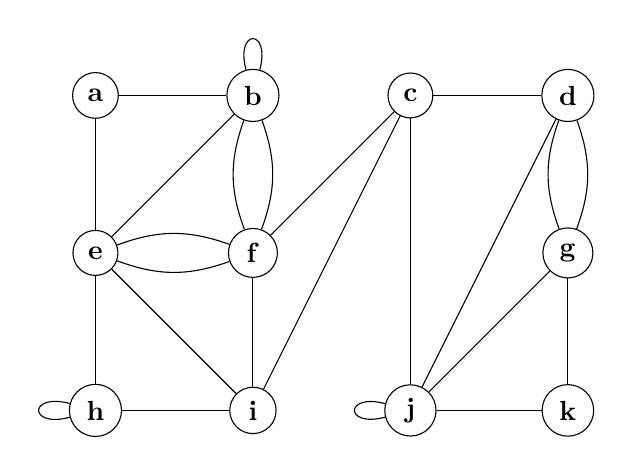
\begin{tikzpicture}[every loop/.style={}]
	
	\node[shape=circle,draw=black] (a) at (0, 4)     {\textbf{a}};
	\node[shape=circle,draw=black] (b) at (2, 4)     {\textbf{b}};
	\node[shape=circle,draw=black] (c) at (4, 4)     {\textbf{c}};
	\node[shape=circle,draw=black] (d) at (6, 4)     {\textbf{d}};
	\node[shape=circle,draw=black] (e) at (0, 2)     {\textbf{e}};
	\node[shape=circle,draw=black] (f) at (2, 2)     {\textbf{f}};
	\node[shape=circle,draw=black] (g) at (6, 2)     {\textbf{g}};
	\node[shape=circle,draw=black] (h) at (0, 0)     {\textbf{h}};
	\node[shape=circle,draw=black] (i) at (2, 0)     {\textbf{i}};
	\node[shape=circle,draw=black] (j) at (4, 0)     {\textbf{j}};
	\node[shape=circle,draw=black] (k) at (6, 0)     {\textbf{k}};
	
	\path[every node/.style={font=\sffamily\small}]
        (b)   edge[loop above] (b);
	\path[every node/.style={font=\sffamily\small}]
        (h)   edge[loop left] (h);
	\path[every node/.style={font=\sffamily\small}]
        (j)   edge[loop left] (j);
	\path[-] (a) edge (b);
	\path[-] (a) edge (e);
	\path[-] (b) edge (e);
	\path[-] (b) edge [bend right=20] (f);
	\path[-] (b) edge [bend left=20] (f);
	\path[-] (c) edge (f);
	\path[-] (c) edge (i);
	\path[-] (c) edge (j);
	\path[-] (c) edge (d);
	\path[-] (d) edge (j);
	\path[-] (d) edge [bend left=20] (g);
	\path[-] (d) edge [bend right=20] (g);
	\path[-] (e) edge [bend left=20] (f);
	\path[-] (e) edge [bend right=20] (f);
	\path[-] (e) edge (h);
	\path[-] (e) edge (i);
	\path[-] (f) edge (i);
	\path[-] (g) edge (j);
	\path[-] (g) edge (k);
	\path[-] (h) edge (i);
	\path[-] (j) edge (k);
	\end{tikzpicture} 
	\caption{Graph G in Q3.}
	\label{g3}
\end{figure}

\begin{itemize}
	\item[\textbf{a.}] Prove whether $G$ has a Euler path or not. \hfill \normalfont{(4 pts)}
	\item[\textbf{b.}] Prove whether $G$ has a Euler circuit or not. \hfill \normalfont{(4 pts)}
	\item[\textbf{c.}] Prove whether $G$ has a Hamiltonian path or not. \hfill \normalfont{(4 pts)}
	\item[\textbf{d.}] Prove whether $G$ has a Hamiltonian circuit or not. \hfill \normalfont{(4 pts)}
\end{itemize}

\section*{Question 4 \hfill \normalfont{(10 pts)}}
Let $K_{m,n}$ denote a complete bipartite graph such that exactly $m$ and $n$ vertices exist in its two disjoints sets of vertices such that $m\,,n\in\mathbb{N}^+$, respectively.
\begin{itemize}
	\item[\textbf{a.}] How many vertices and edges does $K_{m,n}$ have? \hfill \normalfont{(3 pts)}
	\item[\textbf{b.}] Prove that $K_{m,n}$ with odd $m$ and even $n$ does not have a Hamiltonian circuit. \hfill \normalfont{(7 pts)}
\end{itemize}

\pagebreak

\section*{Question 5 \hfill \normalfont{(20 pts)}}
Given the undirected graph $G$ in Figure~\ref{g5}, answer the questions.
\begin{figure}[H]
	\centering
	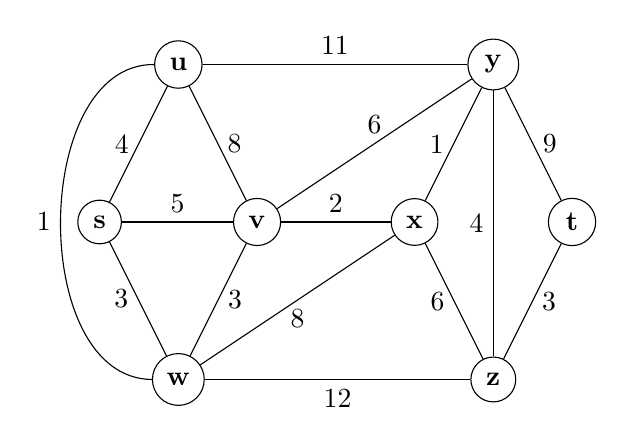
\begin{tikzpicture}
	\node[shape=circle,draw=black] (s) at (1, 2)     {\textbf{s}};
	\node[shape=circle,draw=black] (u) at (2, 4)     {\textbf{u}};
	\node[shape=circle,draw=black] (v) at (3, 2)     {\textbf{v}};
	\node[shape=circle,draw=black] (w) at (2, 0)     {\textbf{w}};
	\node[shape=circle,draw=black] (x) at (5, 2)     {\textbf{x}};
	\node[shape=circle,draw=black] (y) at (6, 4)     {\textbf{y}};
	\node[shape=circle,draw=black] (z) at (6, 0)     {\textbf{z}};
	\node[shape=circle,draw=black] (t) at (7, 2)     {\textbf{t}};

	\path[-] (s) edge node[left]{4} (u);
	\path[-] (s) edge node[above]{5} (v);
	\path[-] (u) edge [bend right=90] node[left]{1} (w);
	\path[-] (u) edge node[above]{11} (y);
	\path[-] (u) edge node[right]{8} (v);
	\path[-] (v) edge node[above]{6} (y);
	\path[-] (v) edge node[above]{2} (x);
	\path[-] (v) edge node[right]{3} (w);
	\path[-] (w) edge node[left]{3} (s);
	\path[-] (w) edge node[below]{8} (x);
	\path[-] (w) edge node[below]{12} (z);
	\path[-] (x) edge node[left]{1} (y);
	\path[-] (x) edge node[left]{6} (z);
	\path[-] (y) edge node[left]{4} (z);
	\path[-] (y) edge node[right]{9} (t);
	\path[-] (z) edge node[right]{3} (t);
		
	\end{tikzpicture} 
	\caption{Graph G in Q5.}
	\label{g5}
\end{figure}
\begin{itemize}
	\item[\textbf{a.}] Find the shortest path from $s$ to $t$ using Dijkstra\textquotesingle s algorithm. Clearly show each step. \hfill \normalfont{(7 pts)}
	\item[\textbf{b.}] Find a minimum spanning tree with root as vertex $x$ using Prim\textquotesingle s algorithm in Section 11.5 of the textbook. Explicitly show every step of computation. \hfill \normalfont{(5 pts)}
	\item[\textbf{c.}] Following edges are added to $G$ one-by-one in order:
	\begin{itemize}
	\item[$\bullet$] $(s, x, 1)$
	\item[$\bullet$] $(t, u, 6)$
	\item[$\bullet$] $(s, z, -3)$
	\item[$\bullet$] $(u, y, 3)$
	\item[$\bullet$] $(w, z, -1)$.
	\end{itemize}
	Without ever calling Prim\textquotesingle s algorithm (or any other algorithm computing minimum spanning trees for graphs from scratch), modify the minimum spanning tree you generated in \textbf{b} so that it maintains to be a minimum spanning tree after the first weighted edge is added to $G$. Repeat this for the remaining edges, each time modifying the previously constructed minimum spanning tree. Separately draw minimum spanning trees of $G$ for each new edge in given order. \hfill \normalfont{(5 pts)}
	\item[\textbf{d.}] Do you think you can iteratively update the shortest path from $s$ to $t$ without calling Dijkstra\textquotesingle s algorithm upon the arrival of listed edges in \textbf{c}? Justify your answer. \hfill \normalfont{(3 pts)}
\end{itemize}

\section*{Question 6 \hfill \normalfont{(15 pts)}} 
Answer options \textbf{a}-\textbf{f} using the binary tree $T$ in Figure~\ref{bintree}. Vertices of $T$ are marked with \texttt{<identifier:key>} annotations. Note that $T$ has the vertex $p$ as its root. Use the notational conventions in your textbook to decide whether a vertex is left or right child of some vertex whenever applicable.
\begin{figure}[H]
	\centering
	\begin{tikzpicture}
	
	\node[shape=circle,draw=black] (p) at (7, 7.5)     {\textbf{p:42}};
	\node[shape=circle,draw=black] (q) at (3, 5)     {\textbf{q:34}};
	\node[shape=circle,draw=black] (r) at (11, 5)     {\textbf{r:75}};
	\node[shape=circle,draw=black] (s) at (1, 2.5)     {\textbf{s:26}};
	\node[shape=circle,draw=black] (t) at (5, 2.5)     {\textbf{t:37}};
	\node[shape=circle,draw=black] (u) at (9, 2.5)    {\textbf{u:63}};
	\node[shape=circle,draw=black] (v) at (13, 2.5)     {\textbf{v:98}};
	\node[shape=circle,draw=black] (w) at (2, 0)     {\textbf{w:33}};
	\node[shape=circle,draw=black] (m) at (4, 0)     {\textbf{m:35}};
	\node[shape=circle,draw=black] (x) at (8, 0)     {\textbf{x:41}};
	\node[shape=circle,draw=black] (y) at (10, 0)     {\textbf{y:71}};
	\node[shape=circle,draw=black] (z) at (14, 0)     {\textbf{z:99}};
	\node[shape=circle,draw=black] (n) at (9, -2.5)     {\textbf{n:61}};
		
	\path[-] (p) edge (q);
	\path[-] (p) edge (r);
	\path[-] (q) edge (t);
	\path[-] (q) edge (s);
	\path[-] (r) edge (u);
	\path[-] (r) edge (v);
	\path[-] (s) edge (w);
	\path[-] (t) edge (m);
	\path[-] (u) edge (x);
	\path[-] (u) edge (y);
	\path[-] (v) edge (z);
	\path[-] (y) edge (n);
	\end{tikzpicture} 
	\caption{Tree T in Q6 options a, b, c, d, e, f.}	
	\label{bintree}
\end{figure}
\begin{itemize}
	\item[\textbf{a.}] What are the number of vertices, the number of edges and the height of $T$? \hfill \normalfont{(1 pt)} 
	\item[\textbf{b.}] Carry out a postorder traversal of $T$ and write down the order in which vertices are visited. \hfill \normalfont{(1 pt)}
	\item[\textbf{c.}] Carry out an inorder traversal of $T$ and write down the order in which vertices are visited. \hfill \normalfont{(1 pt)}
	\item[\textbf{d.}] Carry out a preorder traversal of $T$ and write down the order in which vertices are visited. \hfill \normalfont{(1 pt)}
	\item[\textbf{e.}] Is $T$ a full binary tree? Justify your answer. \hfill \normalfont{(1 pt)}
	\item[\textbf{f.}] Is $T$ a binary search tree using provided keys under comparison with respect to the $\leq$ relation defined on $\mathbb{Z}\times\mathbb{Z}$? Justify your answer. \hfill \normalfont{(1 pt)}
	\item[\textbf{g.}] What is the minimum number of vertices in a full ternary ($m=3$) tree of height $h$ such that $h\in\mathbb{N}^+$? \hfill \normalfont{(1 pt)}
	\item[\textbf{h.}] Construct a binary search tree of minimum height for the following set of integer keys $\{9,\, 3, \,11,\, 15,\, 1,\, 7,\, 22,\, 21,\, 4\}$ employing the $\leq$ relation defined on $\mathbb{Z}\times\mathbb{Z}$. \hfill \normalfont{(2 pts)}
	\item[\textbf{i.}] Using the binary search tree in \textbf{h}, give sequences of vertices that are probed in order to find vertices with key values $2$ and $22$, repsectively. \hfill \normalfont{(1 pt)}
	\item[\textbf{j.}] Construct a binary search tree of maximum height for the following set of binary string keys $\{001,\, 1, \,10,\, 010,\, 0000\}$ using lexicographic ordering (how strings would be listed in a dictionary assuming that 0 comes before 1 in the alphabet) for comparison. \hfill \normalfont{(2 pts)}
	\item[\textbf{k.}] Using the binary search tree in \textbf{j}, give sequences of vertices that are probed so as to find vertices with key values $001$ and $011$, respectively. \hfill \normalfont{(1 pt)}
	\item[\textbf{l.}] Construct a spanning forest for the directed graph $G$ in Figure~\ref{g2} via breadth-first search under the assumption that unvisited vertices are selected for expansion in reverse alphabetic order of vertex identifiers. \hfill \normalfont{(2 pts)}
\end{itemize}

\section{Regulations}
\begin{enumerate}
\item \textbf{}You have to write your answers to the provided sections of the template answer file given. Other than that, you cannot change the provided template answer file. If a latex structure you want to use cannot be compiled with the included packages in the template file, that means you should not use it.
\item \textbf{}Do not write any other stuff, e.g. question definitions, to answers' sections. Only write your answers. Otherwise, you will get 0 from that question.
\item \textbf{Late Submission:} \textbf{Not allowed} 
\item \textbf{Cheating:} \textbf{We have zero tolerance policy for cheating}. People involved in cheating will be punished according to the university regulations.
\item \textbf{Newsgroup:} You must follow the newsgroup (news.ceng.metu.edu.tr) for discussions and possible updates on a daily basis.
\item \textbf{Evaluation:} Your latex file will be converted to pdf and evaluated by course assistants. The .tex file will be checked for plagiarism automatically using "black-box" technique and manually by assistants, so make sure to obey the specifications.
\end{enumerate}


\section{Submission}
Submission will be done via COW. Download the given template file, ``hw5.tex", when you finish your exam upload the .tex file with the same name to COW.  
\\
\noindent
\textbf{Note:} \textbf{You cannot submit any other files.} Don't forget to make sure your .tex file is successfully compiled in Inek machines using the command below. 
\small
\begin{verbatim}
$ pdflatex hw5.tex
\end{verbatim}
\normalsize


\end{document}

